%----------------------- Преамбула -----------------------
\documentclass[ut8x, 14pt, oneside, a4paper]{extarticle}
\usepackage{extsizes} % Для добавления в параметры класса документа 14pt

% Для работы с несколькими языками и шрифтом Times New Roman по-умолчанию
\usepackage[english,russian]{babel}
\usepackage{fontspec}
\setmainfont{Times New Roman}
\usepackage[left=30mm,right=10mm,top=20mm,bottom=20mm]{geometry}
\usepackage{misccorr}
\usepackage{indentfirst}
\usepackage{enumitem}
\usepackage{pdfpages}
\usepackage{placeins}
%\usepackage{ragged2e}
\setlength{\parindent}{1.25cm}
%\setlength{\parskip}{1em} % поменять
%\linespread{1.3}
\renewcommand{\baselinestretch}{1.5}
\setlist{nolistsep} % Отсутствие отступов между элементами \enumerate и \itemize

% Дополнительное окружения для подписей
\usepackage{array}
\newenvironment{signstabular}[1][1]{
	\renewcommand*{\arraystretch}{#1}
	\tabular
}{
	\endtabular
}

% Переопределение стандартных \section, \subsection, \subsubsection по ГОСТу;
% Переопределение их отступов до и после для 1.5 интервала во всем документе
\usepackage{titlesec}

\titleformat{\section}[block]
{\bfseries\normalsize\filcenter}{\thesection}{1em}{}

\titleformat{\subsection}[hang]
{\bfseries\normalsize}{\thesubsection}{1em}{}
\titlespacing\subsection{\parindent}{\parskip}{\parskip}

\titleformat{\subsubsection}[hang]
{\bfseries\normalsize}{\thesubsubsection}{1em}{}
\titlespacing\subsubsection{\parindent}{\parskip}{\parskip}

\newcommand{\specsection}[1]{\section*{#1}\addcontentsline{toc}{section}{#1}}
\newcommand{\specsubsection}[1]{\subsection*{#1}\addcontentsline{toc}{subsection}{#1}}
\newcommand{\specsubsubsection}[1]{\subsubsection*{#1}\addcontentsline{toc}{subsubsection}{#1}}

% Работа с изображениями и таблицами; переопределение названий по ГОСТу
\usepackage{caption}
\captionsetup[figure]{name={Рисунок},labelsep=endash}
\captionsetup[table]{singlelinecheck=false, labelsep=endash}

\usepackage{graphicx}
\usepackage{diagbox} % Диагональное разделение первой ячейки в таблицах

% Цвета для гиперссылок и листингов
\usepackage{color}

% Гиперссылки \toc с кликабельностью
\usepackage[linktoc=all]{hyperref}
\hypersetup{hidelinks}

% Листинги
%\setsansfont{Arial}
%\setmonofont{Courier New}

\usepackage{color} % Цвета для гиперссылок и листингов
%\definecolor{comment}{rgb}{0,0.5,0}
%\definecolor{plain}{rgb}{0.2,0.2,0.2}
%\definecolor{string}{rgb}{0.91,0.45,0.32}
%\hypersetup{citecolor=blue}
\hypersetup{citecolor=black}

\newcommand{\anonsection}[1]{%
	\section*{\centering#1}%
	\addcontentsline{toc}{section}{#1}%
}

\usepackage{pgfplots}
\pgfplotsset{width=7cm,compat=1.9}

\usepackage{caption}
\DeclareCaptionFont{white}{\color{white}}
\DeclareCaptionFormat{listing}{\colorbox{white}{\parbox{\textwidth}{#1#2#3}}}
\captionsetup[lstlisting]{format=listing,justification=raggedright}
\usepackage{listings}
\lstset{
	basicstyle=\footnotesize\ttfamily,
	language=XML, % Или другой ваш язык -- см. документацию пакета
	numbers=left,
	numbersep=5pt,
	tabsize=2,
	extendedchars=\true,
	breaklines=true,
	keywordstyle=\color{blue},
	frame=single,
	showspaces=false,
	showtabs=false,
	xleftmargin=17pt,
	framexleftmargin=17pt,
	framexrightmargin=-5pt,
	framexbottommargin=4pt,
	showstringspaces=false,
	inputencoding=utf8x,
	keepspaces=true
}

%\DeclareCaptionLabelSeparator{line}{\ --\ }
%\DeclareCaptionFont{white}{\color{white}}
%\DeclareCaptionFormat{listing}{\colorbox[cmyk]{0.43,0.35,0.35,0.01}{\parbox{\textwidth}{\hspace{15pt}#1#2#3}}}
%\captionsetup[lstlisting]{
	%	format=listing,
	%	labelfont=white,
	%	textfont=white,
	%	singlelinecheck=false,
	%	margin=0pt,
	%	font={bf,footnotesize},
	%	labelsep=line
	%}

\usepackage{ulem} % Нормальное нижнее подчеркивание
\usepackage{hhline} % Двойная горизонтальная линия в таблицах
\usepackage[figure,table]{totalcount} % Подсчет изображений, таблиц
\usepackage{rotating} % Поворот изображения вместе с названием
\usepackage{lastpage} % Для подсчета числа страниц

\makeatletter
\renewcommand\@biblabel[1]{#1.}
\makeatother

\usepackage{color}
\usepackage[cache=false, newfloat]{minted}
\newenvironment{code}{\captionsetup{type=listing}}{}
\SetupFloatingEnvironment{listing}{name=Листинг}

\usepackage{amsmath}
\usetikzlibrary{datavisualization}
\usetikzlibrary{datavisualization.formats.functions}
\usepackage{csvsimple}

% !TeX TXS-program:compile = txs:///lualatex/[--shell-escape]

\begin{document}
	\begin{titlepage}
		\noindent\begin{minipage}{0.05\textwidth}
			
\includegraphics[scale=0.3]{inc/bmstu.png}
		\end{minipage}
		\hfill
		\begin{minipage}{0.85\textwidth}\raggedleft
			\begin{center}
				\fontsize{12pt}{0.3\baselineskip}\selectfont \textbf{Министерство науки и высшего образования Российской Федерации \\ Федеральное государственное бюджетное образовательное учреждение \\ высшего образования \\ <<Московский государственный технический университет \\ имени Н.Э. Баумана \\ (национальный исследовательский университет)>> \\ (МГТУ им. Н.Э. Баумана)}
			\end{center}
		\end{minipage}
		
		\begin{center}
			\fontsize{12pt}{0.1\baselineskip}\selectfont
			\noindent\makebox[\linewidth]{\rule{\textwidth}{4pt}} \makebox[\linewidth]{\rule{\textwidth}{1pt}}
		\end{center}
		
		\begin{flushleft}
			\fontsize{12pt}{0.8\baselineskip}\selectfont 
			
			ФАКУЛЬТЕТ \uline{<<\textbf{Информатика и системы управления}>> \hfill}
			
			КАФЕДРА \uline{\mbox{\hspace{4mm}} <<\textbf{Программное обеспечение ЭВМ и информационные технологии}>> \hfill}
		\end{flushleft}
		
		\vfill
		
		\begin{center}
			\fontsize{20pt}{\baselineskip}\selectfont
			
			\textbf{РАСЧЕТНО-ПОЯСНИТЕЛЬНАЯ ЗАПИСКА}
			
			\textbf{\textit{К КУРСОВОЙ РАБОТЕ}}
			
			\textbf{\textit{НА ТЕМУ:}}
		\end{center}
		
		\begin{center}
			\fontsize{18pt}{0.6cm}\selectfont 
			
			\textit{<<Разработка базы данных для хранения информации о репетиционных базах>>}
			
		\end{center}
		
		\vfill
		
		\begin{table}[h!]
			\fontsize{12pt}{0.7\baselineskip}\selectfont
			
			\begin{signstabular}[0.55]{p{7.25cm} >{\centering\arraybackslash}p{4cm} >{\centering\arraybackslash}p{4cm}}
				Студент \uline{~~ИУ7-66Б~~} & \uline{\mbox{\hspace*{4cm}}} & \uline{\hfill \textbf{А. А. Петрова} \hfill} \\
				\scriptsize \hspace*{2cm}(Группа)	& \scriptsize (Подпись, дата) & \scriptsize (И.О. Фамилия)
			\end{signstabular}
			
			\vspace{\baselineskip}
			
			\begin{signstabular}[0.55]{p{7.25cm} >{\centering\arraybackslash}p{4cm} >{\centering\arraybackslash}p{4cm}}
				Руководитель & \uline{\mbox{\hspace*{4cm}}} & \uline{\hfill \textbf{М. В. Филиппов} \hfill} \\
				& \scriptsize (Подпись, дата) & \scriptsize (И.О. Фамилия)
			\end{signstabular}
		\end{table}
		
		\vfill
		
		\begin{center}
			\normalsize \textit{2022 г.}
		\end{center}
	\end{titlepage}

\pagenumbering{gobble}
%\include{tex/tz.tex}
\normalsize
\pagenumbering{arabic}
\setcounter{page}{2}

\section*{РЕФЕРАТ}

Расчетно-пояснительная записка 36 с., 10 рис., 5 табл., 7 ист., 5 прил.

Объектом разработки в данной работе является база данных, содержащая информацию о репетиционных базах, соответствующих им комнатах и оборудовании, с целью предоставить возможность пользователям искать необходимые комнаты и бронировать свои репетиции. Цель данной работы – реализовать приложение, содержащее информацию о репетиционных базах. В приложении, работающем с этой БД, должна быть возможность для музыканта бронировать или отменять свои репетиции, а для владельца реп. базы - отслеживать записи на свою реп. базу.

Чтобы достигнуть поставленной цели, требуется решить следующие задачи:
\begin{itemize}
	\item формализовать задание, определить необходимый функционал;
	\item провести анализ СУБД;
	\item описать структуру БД;
	\item создать и заполнить БД;
	\item разработать ПО, которое позволит пользователю-музыканту бронировать и отменять свои репетиции, а владельцу отслеживать их;
	\item провести исследование зависимости времени выполнения запроса от числа записей в таблице.
\end{itemize}

Поставленная цель достигнута: в ходе курсового проекта была разработана база данных, хранящая информацию о репетиционных точках. При этом при разработке в качестве СУБД использовался PostgreSQL, а в качестве языка программирования – Python 3.7.

Дальнейшее развитие проекта подразумевает:
\begin{itemize}
	\item добавление фотографий комнат в блок информации о них;
	\item добавление календаря для более удобного бронирования репетиций;
	\item добавление возможности бронировать не только репетиционные базы, но и другие творческие площадки;
	\item добавление возможности администраторам блокировать пользователей;
	\item создание мобильной версии приложения.
\end{itemize}

КЛЮЧЕВЫЕ СЛОВА

\textit{базы данных, разработка ПО, репетиционные базы, бронирование репетиций, postgresql, python.}

\clearpage

\renewcommand{\contentsname}{\normalsize\bfseries\centering СОДЕРЖАНИЕ}
\tableofcontents
\clearpage


\specsection{Введение}

Проблема поиска места для репетиций является актуальной для любого музыканта, тем более группы. В крупных городах есть достаточно много репетиционных баз (далее: реп. баз). Все они имеют разные цены и характеристики. Поэтому существует потребность в приложении, которое собирало бы воедино всю имеющуюся информацию о различных репетиционных базах, таким образом освобождая музыкантов от необходимости вручную искать и изучать каждую реп. базу, заходить на их сайты, звонить лично, чтобы забронировать репетицию и т. д.

Цель данной работы – реализовать приложение, содержащее информацию о репетиционных базах. В приложении, работающем с этой БД, должна быть возможность для музыканта бронировать или отменять свои репетиции, а для владельца реп. базы - отслеживать записи на свою реп. базу.

Чтобы достигнуть поставленной цели, требуется решить следующие задачи:
\begin{itemize}
	\item формализовать задание, определить необходимый функционал;
	\item провести анализ СУБД;
	\item описать структуру БД;
	\item создать и заполнить БД;
	\item разработать ПО, которое позволит пользователю-музыканту бронировать и отменять свои репетиции, а владельцу отслеживать их;
	\item провести исследование зависимости времени выполнения запроса от числа записей в таблице.
\end{itemize}
\section{Аналитическая часть}

\subsection{Анализ задачи и существующих решений}

Необходимо разработать программу для отображения информации о репетиционных базах с возможностью для музыканта бронировать или отменять свои репетиции, а для владельца реп. базы - отслеживать записи на свою реп. базу.

На сегодняшний день существует всего два подобных приложения:
\begin{itemize}
	\item MUSbooking
	
	Это наиболее известное и популярное приложение по бронированию творческих площадок.
	
	Его основные преимущества: возможность бронирования любых творческих площадок и возможность бронирования в других городах России (не только в Москве).
	
	Основной недостаток: нельзя посмотреть сразу весь список зарегистрированных реп. баз в текущем городе. Список доступных реп. баз можно посмотреть только после указания конкретного времени репетиции, что крайне неудобно в определённых ситуациях.
	
	\item TONESKY
	
	Основное преимущество: возможность заранее посмотреть весь список зарегистрированных реп. баз.
	
	Из недостатков: отсутствие поиска по реп. базам, отсутствие цены на превью (т. е., чтобы посмотреть цену, надо зайти «вглубь» и посмотреть подробную информацию), ориентация только на Москву (не существенно в рамках моей задачи).
\end{itemize}

\subsection{Формализация данных}

База данных должна хранить информацию о:

\begin{itemize}
	\item репетиционной базе и её комнатах;
	\item оборудовании;
	\item пользователях (музыкантах и владельцах) и об их забронированных репетициях или реп. базах соответственно.
\end{itemize}

\begin{figure}[h!]
	\begin{center}
		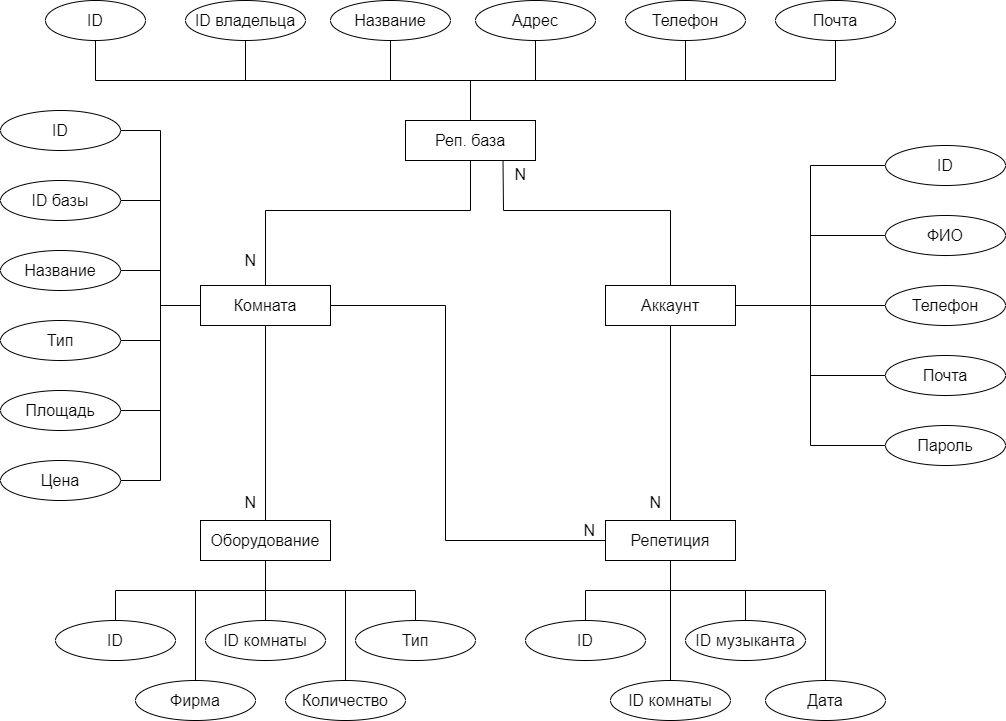
\includegraphics[scale=0.45]{inc/img/ER_Chena.png}
	\end{center}
	\captionsetup{justification=centering}
	\caption{ER-диаграмма разрабатываемой базы данных}
	\label{img:er-diagram}
\end{figure}

\begin{table}[!h]
	\captionsetup{justification=centering}
	\caption{\label{tab:data} Категории и сведения о данных}
	\begin{center}
		\begin{tabular}{|p{0.2\textwidth}|p{0.7\textwidth}|}
			\hline
			\textbf{Категория} & \textbf{Сведения}\\
			\hline
			Реп. база & Название, адрес, телефон, почта, кому принадлежит \\
			\hline
			Комната & Название, тип (вокал/группа и т. д.), площадь, стоимость за 3 часа, к какой репбазе относится \\
			\hline
			Оборудование в комнате & Тип (усилитель/ударные/микрофон и т. д.), бренд, количество, к какой комнате относится \\
			\hline
			Аккаунт & ФИО, телефон, почта \\
			\hline
			Репетиция & Время, какой музыкант (аккаунт), какая комната \\
			\hline
		\end{tabular}
	\end{center}
\end{table}

\newpage

\subsection{Типы пользователей}

Из задачи ясно, что есть два типа пользователей: обычный музыкант и владелец реп. базы. Помимо этого, будет также выделена роль администратора приложения. Для всех троих будет нужна авторизация.

\begin{figure}[h!]
	\begin{center}
		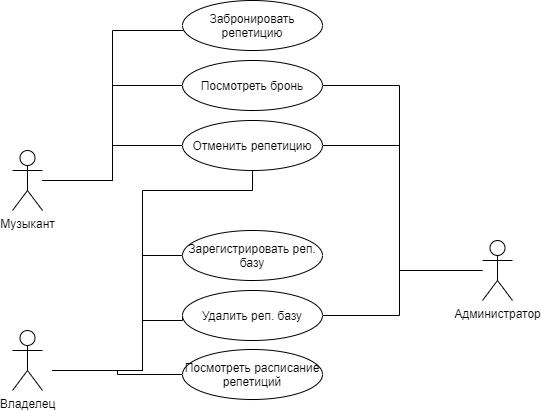
\includegraphics[scale=0.7]{inc/img/Use-Case.png}
	\end{center}
	\captionsetup{justification=centering}
	\caption{Use-case диаграмма приложения}
\end{figure}

\begin{table}[!h]
	\captionsetup{justification=centering}
	\caption{Типы пользователей и их полномочия}
	\begin{center}
		\begin{tabular}{|p{0.25\textwidth}|p{0.65\textwidth}|}
			\hline
			\textbf{Тип пользователя} & \textbf{Полномочия}\\
			\hline
			Музыкант & Бронирование репетиций, отмена репетиций, просмотр брони \\
			\hline
			Владелец & Добавление репбазы, удаление своей репбазы, просмотр записей на репетиции, отмена репетиций \\
			\hline
			Администратор & Удаление репбазы, отмена репетиций, просмотр бронирований \\
			\hline
		\end{tabular}
	\end{center}
\end{table}

\subsection{Классификации СУБД}

Система управления базами данных (СУБД) – совокупность программных и лингвистических средств общего или специального назначения, обеспечивающих управление созданием и использованием баз данных \cite{subd_opr}.

Основными функциями СУБД являются:
\begin{itemize}
	\item управление данными на внешней памяти;
	\item управление данными в оперативной памяти с использованием дискового кэша;
	\item журнализация изменений, резервное копирование и восстановление базы данных после сбоев;
	\item поддержка языков БД.
\end{itemize}

\textbf{Классификации СУБД:}

По модели данных:
\begin{itemize}
	\item дореляционные;
	
	\textbf{Иерархические.} Это модель данных, где используется представление базы данных в виде древовидной (иерархической) структуры, состоящей из объектов (данных) различных уровней.
	
	\textbf{Сетевые.} Это логическая модель данных, являющаяся расширением иерархического подхода, строгая математическая теория, описывающая структурный аспект, аспект целостности и аспект обработки данных в сетевых базах данных.
	
	Разница между иерархической моделью данных и сетевой состоит в том, что в иерархических структурах запись-потомок должна иметь в точности одного предка, а в сетевой структуре данных у потомка может иметься любое число предков.
	
	\item реляционные.
	
	Реляционная модель данных является совокупностью данных и состоит из набора двумерных таблиц. При табличной организации отсутствует иерархия элементов. Таблицы состоят из строк – записей и столбцов – полей. На пересечении строк и столбцов находятся конкретные значения. Для каждого поля определяется множество его значений. За счет возможности просмотра строк и столбцов в любом порядке достигается гибкость выбора подмножества элементов.
	
	Реляционная модель является удобной и наиболее широко используемой формой представления данных.
	
\end{itemize}

Модель данных — это абстрактное, самодостаточное, логическое определение объектов, операторов и прочих элементов, в совокупности составляющих абстрактную машину доступа к данным, с которой взаимодействует пользователь. Эти объекты позволяют моделировать структуру данных, а операторы — поведение данных \cite{data_model}.

По степени распределённости:
\begin{itemize}
	\item локальные (все части локальной СУБД размещаются на одном компьютере);
	\item распределённые (части СУБД могут размещаться не только на одном, но на двух и более компьютерах).
\end{itemize}

По способу доступа к БД:
\begin{itemize}
	\item файл-серверные;
	
	В файл-серверных СУБД файлы данных располагаются централизованно на файл-сервере. СУБД располагается на каждом клиентском компьютере (рабочей станции). Доступ СУБД к данным осуществляется через локальную сеть. Синхронизация чтений и обновлений осуществляется посредством файловых блокировок.
	
	Преимуществом этой архитектуры является низкая нагрузка на процессор файлового сервера.
	
	Недостатки: потенциально высокая загрузка локальной сети; затруднённость или невозможность централизованного управления; затруднённость или невозможность обеспечения таких важных характеристик, как высокая надёжность, высокая доступность и высокая безопасность. Применяются чаще всего в локальных приложениях, которые используют функции управления БД; в системах с низкой интенсивностью обработки данных и низкими пиковыми нагрузками на БД.
	
	На данный момент файл-серверная технология считается устаревшей, а её использование в крупных информационных системах — недостатком  \cite{file_server}.
	
	Пример: Microsoft Access.
	
	\item клиент-серверные;
	
	Клиент-серверная СУБД располагается на сервере вместе с БД и осуществляет доступ к БД непосредственно, в монопольном режиме. Все клиентские запросы на обработку данных обрабатываются клиент-серверной СУБД централизованно.
	
	Недостаток клиент-серверных СУБД состоит в повышенных требованиях к серверу.
	
	Достоинства: потенциально более низкая загрузка локальной сети; удобство централизованного управления; удобство обеспечения таких важных характеристик, как высокая надёжность, высокая доступность и высокая безопасность.
	
	Примеры: Oracle Database, MS SQL Server, PostgreSQL, MySQL.
	
	\item встраиваемые.
	
	СУБД, которая может поставляться как составная часть некоторого программного продукта, не требуя процедуры самостоятельной установки. Встраиваемая СУБД предназначена для локального хранения данных своего приложения и не рассчитана на коллективное использование в сети.
	
	Физически встраиваемая СУБД чаще всего реализована в виде подключаемой библиотеки. Доступ к данным со стороны приложения может происходить через SQL либо через специальные программные интерфейсы.
	
	Примеры: SQLite, Microsoft SQL Server Compact.
	
\end{itemize}

\subsection*{Выводы}

В этом разделе была проанализирована поставленная задача и уже существующие решения. А также были формализованы данные, типы пользователей и их полномочия. После чего были рассмотрены разные типы СУБД и их функции.



\section{Конструкторская часть}

\subsection{Проектирование БД}

База данных должна хранить представленные в таблице \ref{tab:data} данные. Исходя из этого, в проектируемой базе данных можно выделить следующие таблицы:
\begin{itemize}
	\item таблица с реп. базами (rehbase);
	\item таблица с комнатами реп. баз (room);
	\item таблица с оборудованием в комнатах (equipment);
	\item таблица с аккаунтами пользователей (account);
	\item таблица с забронированными репетициями (rehearsal).
\end{itemize}

Таблица rehbase должна содержать информацию о:
\begin{itemize}
	\item id – идентификатор реп. базы (PK);
	\item name – название реп. базы (text);
	\item address – адрес реп. базы (text);
	\item phone – номер телефона для связи (text);
	\item mail – электронная почта для связи (text);
	\item ownerid – id владельца реп. базы (связь с таблицей account) (FK, один-ко-многим).
\end{itemize}

Таблица room должна содержать информацию о:
\begin{itemize}
	\item id – идентификатор комнаты (PK);
	\item name – название комнаты (text);
	\item type – тип комнаты (text);
	\item area – площадь комнаты (integer);
	\item cost – стоимость репетиции в этой комнате за 3 часа (integer);
	\item baseid – id реп. базы, которой принадлежит комната (связь с таблицей rehbase) (FK, один-ко-многим).
\end{itemize}

Таблица equipment должна содержать информацию о:
\begin{itemize}
	\item id – идентификатор оборудования (PK);
	\item type – тип оборудования (text);
	\item brand – фирма оборудования (text);
	\item amount – количество оборудования такого типа в соответствующей комнате (integer);
	\item roomid – id комнаты, в которой находится это оборудование (связь с таблицей room) (FK, один-ко-многим).
\end{itemize}

Таблица account должна содержать информацию о:
\begin{itemize}
	\item id – идентификатор пользователя (PK);
	\item fio – ФИО пользователя (text);
	\item phone – номер телефона пользователя (text);
	\item mail – электронная почта пользователя (text);
	\item password – пароль от аккаунта (text);
	\item type – тип пользователя (text).
\end{itemize}

Таблица rehearsal должна содержать информацию о:
\begin{itemize}
	\item id – идентификатор репетиции (PK);
	\item rehdate – дата и время репетиции (timestamp);
	\item musicianid – id музыканта, забронировавшего репетицию (связь с таблицей account) (FK, один-ко-многим);
	\item roomid – id комнаты, в которой забронирована репетиция (связь с таблицей room) (FK, один-ко-многим).
\end{itemize}

\begin{figure}[h!]
	\begin{center}
		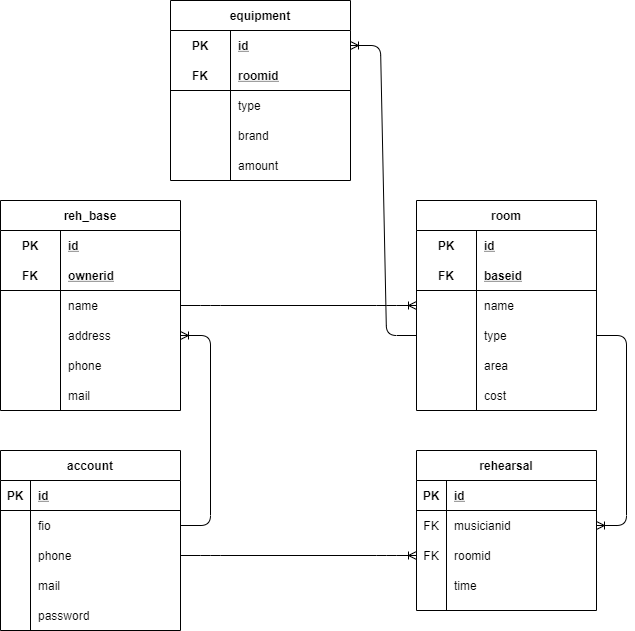
\includegraphics[scale=0.5]{inc/img/ER_DB.png}
	\end{center}
	\captionsetup{justification=centering}
	\caption{ER диаграмма проектируемой БД}
	\label{img:er}
\end{figure}

\newpage

\subsection{Требования к программе}

Разрабатываемое ПО должно предоставлять следующие возможности:
\begin{itemize}
	\item регистрация нового пользователя;
	\item авторизация пользователя;
	\item вывод списка комнат, доступных для бронирования;
	\item вывод подробной информации о каждой комнате;
	\item бронь комнаты на соответствующее время;
	\item отмена брони;
	\item вывод уже забронированных (будущих) репетиций;
	\item вывод зарегистрированных реп. баз для данного аккаунта;
	\item регистрация новой реп. базы;
	\item добавление комнаты в зарегистрированную реп. базу;
	\item добавление оборудования в соответствующую комнату;
	\item вывод всех будущих репетиций на соответствующей реп. базе;
	\item удаление реп. базы;
	\item поиск по имени реп. базы;
	\item поиск по дате и времени репетиции.
\end{itemize}

Ограничения, в рамках которых будет работать программа:
\begin{itemize}
	\item аккаунт нельзя удалить;
	\item нельзя зарегистрироваться стандартным способом в качестве администратора (администраторы добавляются «вручную» на уровне БД);
	\item для обновления информации нужно закрыть соответствующее окно и снова его открыть;
	\item для выхода из аккаунта нужно закрыть окно;
	\item пароль от аккаунта хранится в БД в обычном виде, без шифрования;
	\item календарь для бронирования репетиций не предоставляется.
\end{itemize}

\subsection{Структура ПО}

Всё проектируемое ПО можно разделить на две основные части:
\begin{itemize}
	\item frontend (часть приложения, с которой непосредственно взаимодействует пользователь, отображение данных);
	\item backend (взаимодействие с базой данных).
\end{itemize}

Структура frontend части в свою очередь будет основана на паттерне MVC (Model, View, Controller).

Таким образом, проект будет разделён на несколько файлов:
\begin{itemize}
	\item connect – взаимодействие непосредственно с БД;
	\item gui – здесь будут находиться модели и контроллеры frontend части;
	\item отдельные файлы для каждого окна итогового приложения, предоставляющие интерфейс пользователю (т. е. отвечающие за view часть).
\end{itemize}

Файл connect будет состоять из набора следующих функций:
\begin{itemize}
	\item connect\_* – для подключения к БД с соответствующей ролью;
	\item функции для формирования и посылки запросов к БД.
\end{itemize}

Файл gui в свою очередь будет состоять из набора классов, каждый из которых будет соответствовать определённому окну приложения.

На рисунке \ref{img:classes} представлена диаграмма классов разрабатываемого приложения.

\begin{figure}[h!]
	\begin{center}
		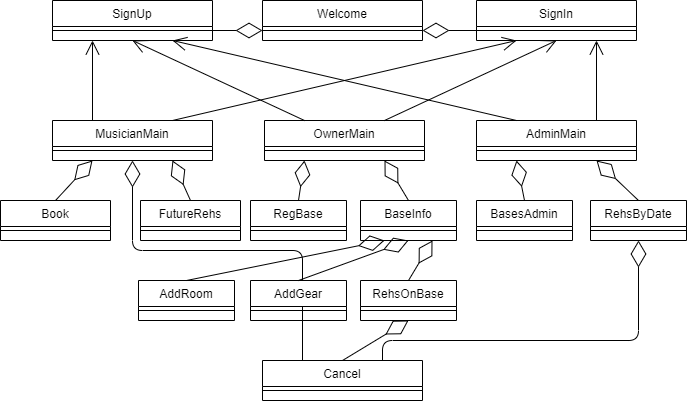
\includegraphics[scale=0.6]{inc/img/Classes.png}
	\end{center}
	\captionsetup{justification=centering}
	\caption{Диаграмма классов}
	\label{img:classes}
\end{figure}

\subsection{Способы и этапы тестирования}

Для проверки работоспособности ПО будет применяться функциональное тестирование.

Тестирование ПО будет разделено на следующие этапы:
\begin{itemize}
	\item регистрация нового пользователя (как музыканта, так и владельца);
	\item попытка зарегистрироваться ещё раз с той же почтой;
	\item попытка авторизоваться с неправильной почтой или паролем;
	\item авторизация в качестве музыканта;
	\begin{itemize}
		\item бронирование репетиции;
		\item попытка забронировать репетицию в уже забронированной на это время комнате;
		\item просмотр своих будущих репетиций;
		\item отмена брони;
		\item попытка забронировать репетицию «в прошлом»;
	\end{itemize}
	\item авторизация в качестве владельца;
	\begin{itemize}
		\item регистрация новой реп. базы;
		\item попытка зарегистрировать уже существующую реп. базу (с той же почтой либо с тем же названием и адресом);
		\item добавление комнаты в реп. базу;
		\item попытка добавить уже существующую комнату (с тем же названием);
		\item добавление оборудования в комнату;
		\item попытка добавить оборудование в несуществующую комнату;
		\item попытка повторно добавить то же самое оборудование в ту же самую комнату;
		\item просмотр предстоящих репетиций на соответствующей реп. базе;
		\item удаление реп. базы;
	\end{itemize}
	\item авторизация в качестве администратора;
	\begin{itemize}
		\item поиск реп. баз по названию (успешный);
		\item попытка найти несуществующую реп. базу;
		\item поиск репетиций по дате (успешный);
		\item попытка найти несуществующую репетицию.
	\end{itemize}
\end{itemize}

\subsection*{Выводы}

На основе теоретических данных, полученных в аналитическом разделе, были спроектированы база данных и приложение. А также были приведены: требования к программе, способы и этапы тестирования и диаграмма классов.


\section{Технологическая часть}

\subsection{Выбор СУБД}

В таблице \ref{tab:subd} произведено сравнение наиболее популярных СУБД, которые могут быть использованы для реализации хранения данных в разрабатываемом программном продукте.

\begin{table}[!h]
	\captionsetup{justification=centering}
	\caption{\label{tab:subd} Особенности различных СУБД}
	\begin{center}
		\begin{tabular}{|p{0.15\textwidth}|p{0.2\textwidth}|p{0.15\textwidth}|p{0.15\textwidth}|p{0.15\textwidth}|}
			\hline
			\textbf{Особенность} & \textbf{MySQL} & \textbf{PostgreSQL} & \textbf{MS SQL Server} & \textbf{Oracle Database} \\
			\hline
			Open source & GNU GPL с открытым исходным кодом & Открытый исходный код & Коммерческая & Коммерческая\\
			\hline
			Соответствие ACID & Частичное (зависит от версии) \cite{acid} & Полное & Полное & Полное\\
			\hline
			NoSQL / JSON & Поддержка некоторых функций & JSON, NoSQL & JSON, NoSQL & JSON, NoSQL\\
			\hline
			Поддержка MERGE & Да & Нет & Да & Да\\
			\hline
		\end{tabular}
	\end{center}
\end{table}

Таким образом, для реализации проекта в качестве СУБД будет использоваться PostgreSQL, так как он является свободно распространяемым и удовлетворяет всем необходимым требованиям в рамках поставленной задачи.

\subsection{Выбор ЯП и среды программирования}

Для реализации проекта в качестве языка программирования был выбран язык Python, так как:
\begin{itemize}
	\item этот язык поддерживает работу с PostgreSQL (в моём случае для этого будет использоваться библиотека psycopg2);
	\item данный язык является полностью объектно-ориентированным (всё является объектами) \cite{python}, что позволяет в полной мере использовать классы при написании программы;
	\item в этом языке присутствует PyQt (набор расширений графического фреймворка Qt для языка программирования Python, выполненный в виде расширения Python \cite{pyqt}), позволяющий легко создавать графический интерфейс для приложения.
\end{itemize}

В качестве среды разработки был выбран PyCharm по следующим причинам:
\begin{itemize}
	\item наличие бесплатной версии Community Edition;
	\item множество удобств, облегчающих процесс написания и отладки кода.
\end{itemize}

\subsection{Детали реализации}
В приложениях А -- Б представлен пример реализации frontend части приложения.

В приложении В представлена реализация соединения с базой данных в соответствии с ролевой моделью.

Помимо этого, на уровне базы данных была реализована процедура, необходимая для удаления реп. базы (приложения Г – Д).

%\subsection{Интерфейс программы}

На рисунках ниже представлен основной интерфейс приложения.

\begin{figure}[h!]
	\begin{center}
		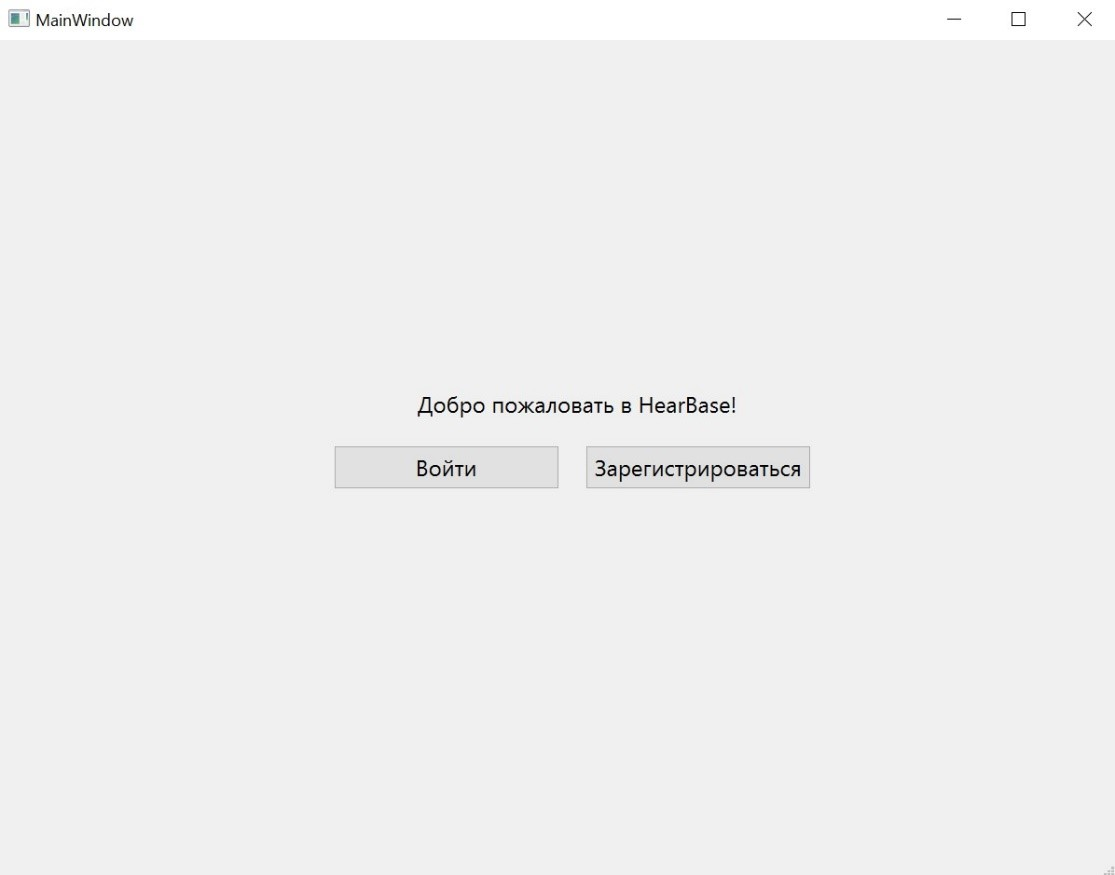
\includegraphics[scale=1]{jpg/Welcome.jpg}
	\end{center}
	\captionsetup{justification=centering}
	\caption{Окно с приглашением}
\end{figure}

\newpage

\begin{figure}[h!]
	\begin{center}
		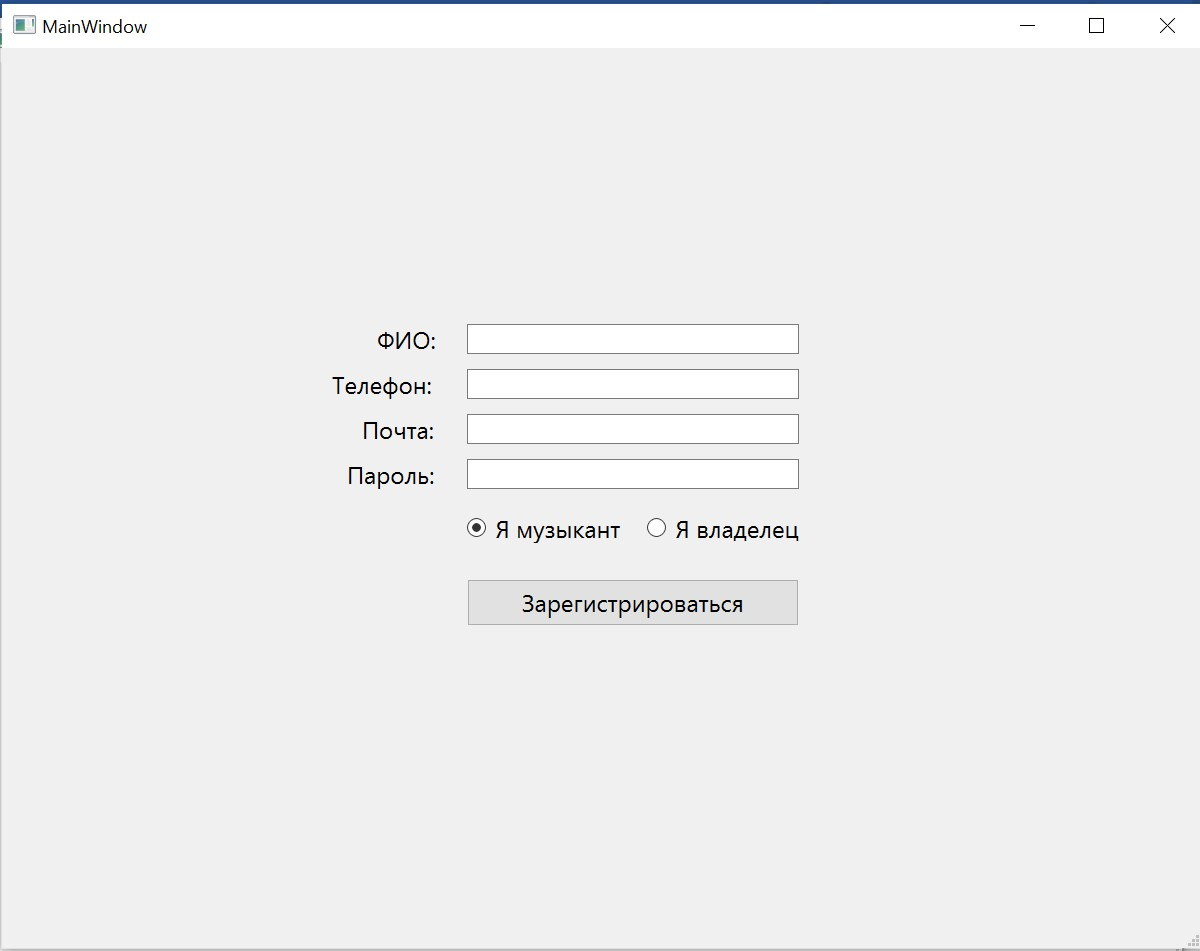
\includegraphics[scale=0.4]{jpg/Reg.jpg}
	\end{center}
	\captionsetup{justification=centering}
	\caption{Окно регистрации}
\end{figure}

\begin{figure}[h!]
	\begin{center}
		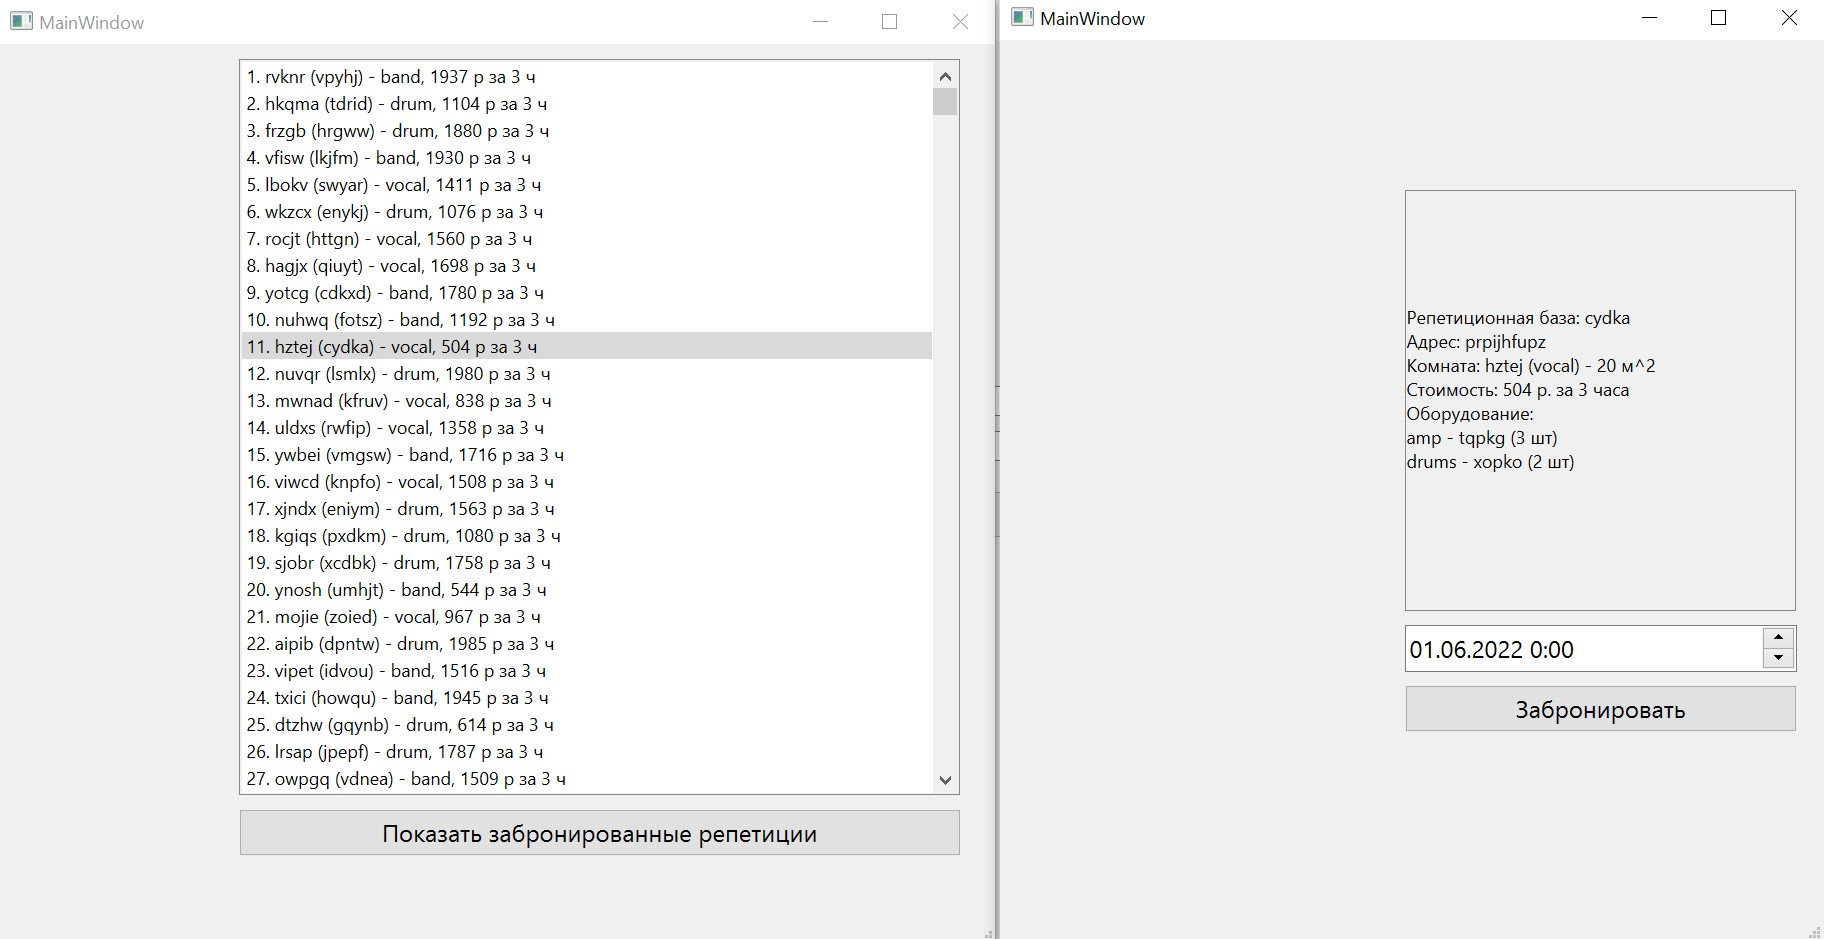
\includegraphics[scale=0.35]{jpg/Musician.jpg}
	\end{center}
	\captionsetup{justification=centering}
	\caption{Интерфейс при входе в качестве музыканта}
\end{figure}

\newpage

\begin{figure}[h!]
	\begin{center}
		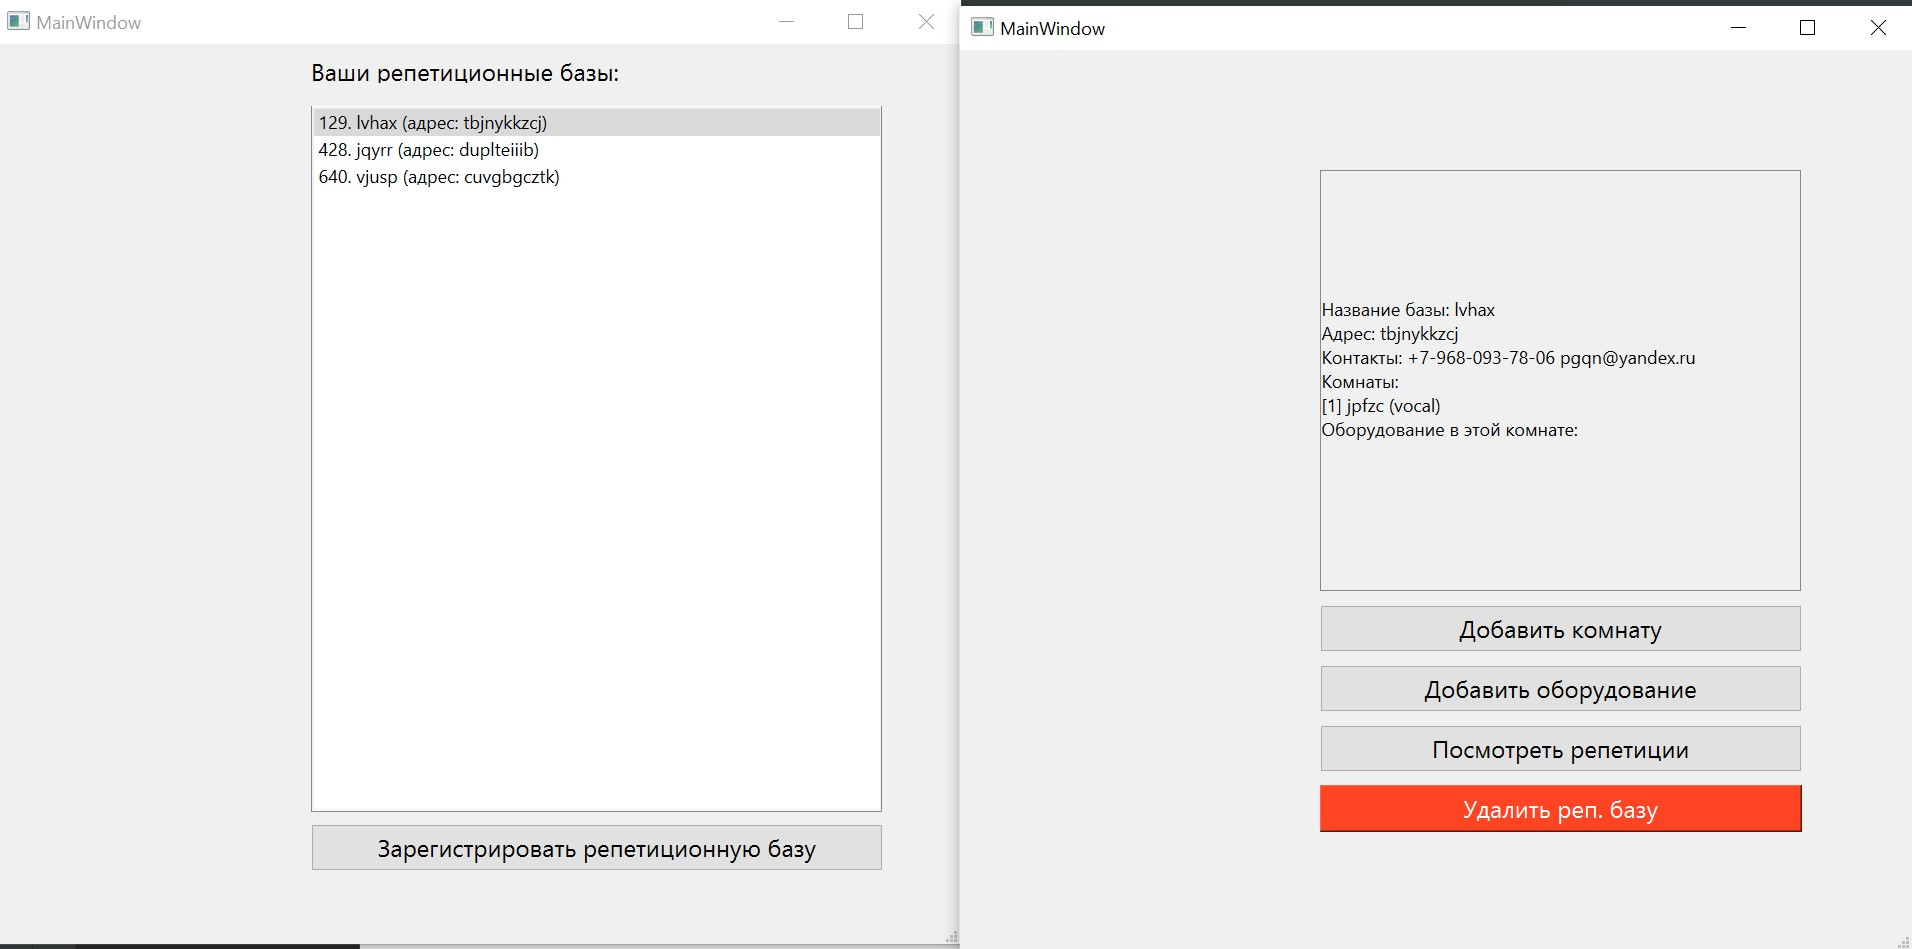
\includegraphics[scale=0.3]{jpg/Owner.jpg}
	\end{center}
	\captionsetup{justification=centering}
	\caption{Интерфейс при входе в качестве владельца}
\end{figure}

\begin{figure}[h!]
	\begin{center}
		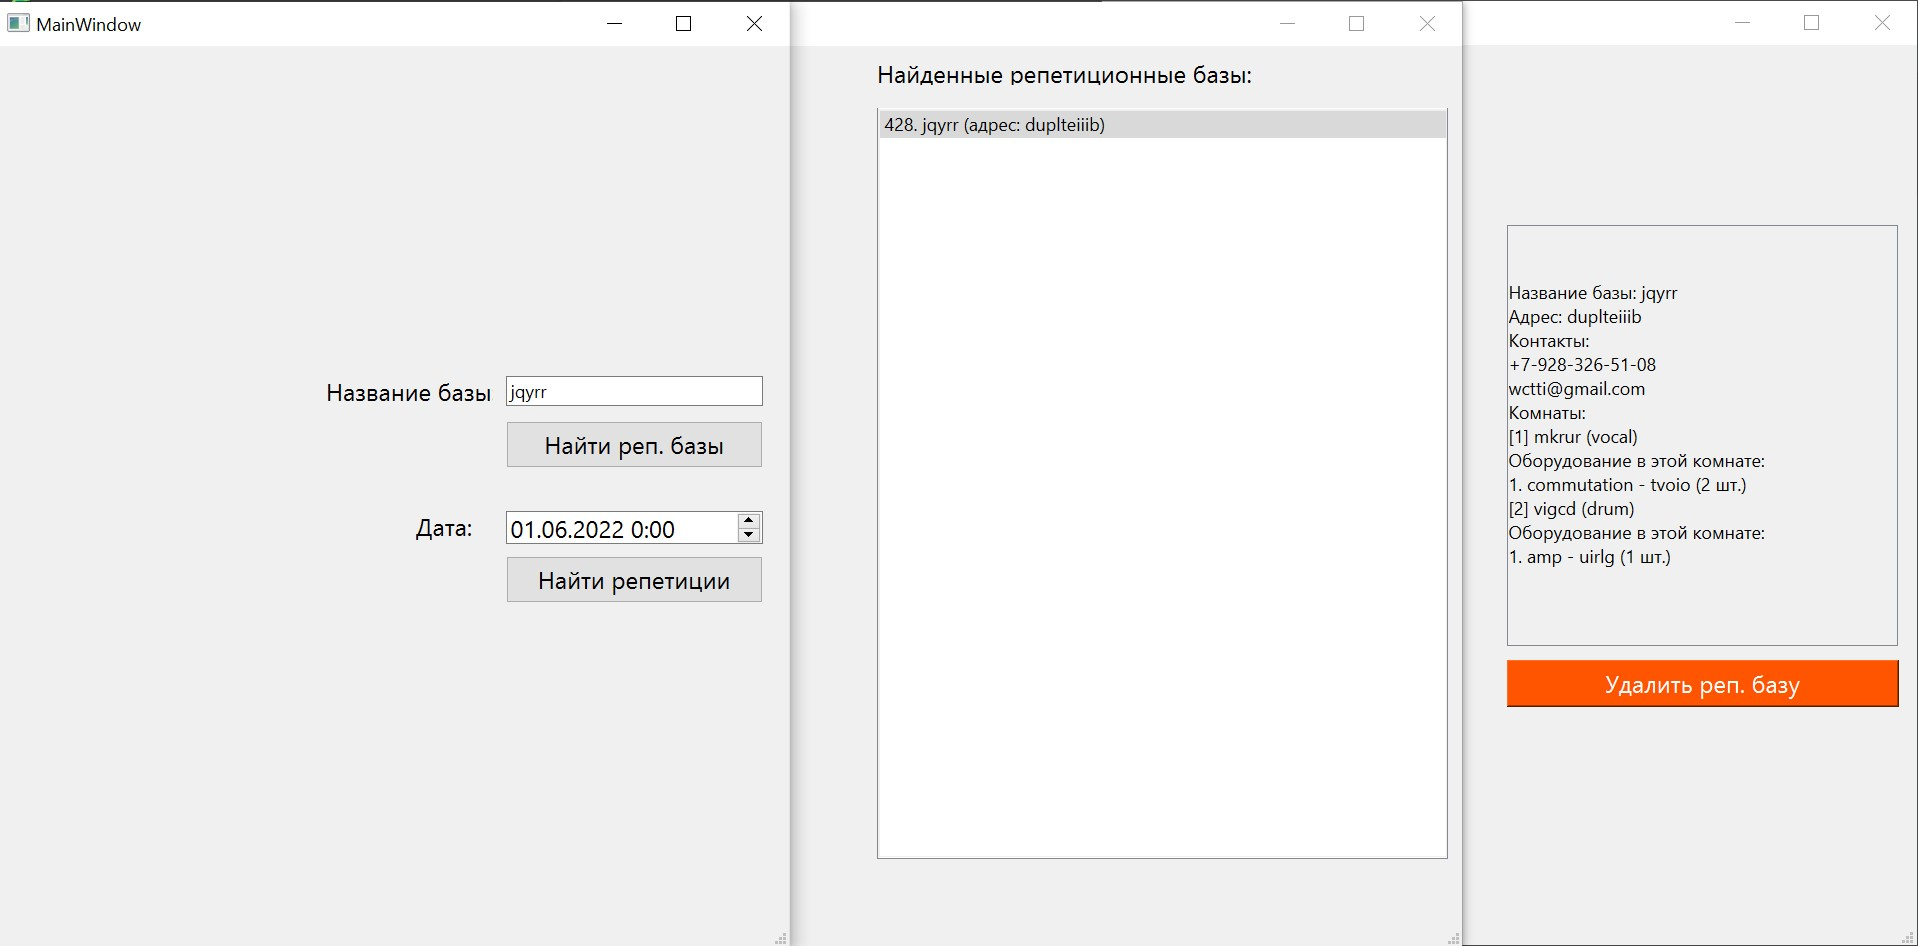
\includegraphics[scale=0.3]{jpg/Admin.jpg}
	\end{center}
	\captionsetup{justification=centering}
	\caption{Интерфейс при входе в качестве администратора}
\end{figure}

\newpage

\subsection*{Выводы}

В данном разделе были выбраны СУБД, язык программирования и среда разработки.

В качестве СУБД выбрана PostgreSQL, так как она:
\begin{itemize}
	\item свободно распространяемая;
	\item полностью соответствует требованиям ACID;
	\item поддерживает все необходимые в рамках поставленной задачи функции (такие, как вложенные селекты, транзакции, триггеры, процедуры).
\end{itemize}

В качестве языка программирования был выбран Python, так как он:
\begin{itemize}
	\item поддерживает работу с PostgreSQL;
	\item объектно-ориентированный;
	\item обладает необходимыми расширениями для работы с графическим интерфейсом.
\end{itemize}

В качестве среды разработки был выбран PyCharm, так как он:
\begin{itemize}
	\item имеет свободно распространяемую версию;
	\item содержит множество удобств для написания и отладки кода, а также для работы с СУБД.
\end{itemize}

Помимо этого, в данном разделе был разработан и протестирован исходный код программы. Программа тестировалась в соответствии с этапами, приведёнными в разделе 2.4. Все тесты были успешно пройдены.

\section{Исследовательская часть}

\subsection{Цель эксперимента}

Целью эксперимента является выявление зависимости времени выполнения запроса от числа записей в таблице, а также от вида самого запроса.

Чтобы достигнуть поставленной цели, требуется решить следующие задачи:
\begin{itemize}
	\item выбрать запросы, время выполнения которых будет замеряться;
	\item измерить время для каждого запроса и каждого числа записей в таблице;
	\item построить график зависимости времени от размеров таблиц и запросов;
	\item проанализировать полученные результаты.
\end{itemize}

Ниже приведены технические характеристики устройства, на котором будет проводиться эксперимент:
\begin{itemize}
	\item операционная система: Windows 10 64-bit Home;
	\item оперативная память: 8 GB;
	\item процессор: 11th Gen Intel(R) Core(TM) i3-1115G4 @ 3.00GHz \cite{intel}.
\end{itemize}

\subsection{Постановка эксперимента}

При эксперименте использовались запросы двух видов.

Первый вариант запроса:

\begin{lstlisting}
	select *
	from rehearsal join room on rehearsal.roomid = room.id
	join account on rehearsal.musicianid = account.id
	join reh_base on room.baseid = reh_base.id
\end{lstlisting}

Второй вариант запроса:

\begin{lstlisting}
	select rehearsal.rehdate, room.name, room.type, room.area, room.cost,
	reh_base.name, reh_base.address, reh_base.phone, reh_base.mail
	from rehearsal join room on rehearsal.roomid = room.id
	join account on rehearsal.musicianid = account.id
	join reh_base on room.baseid = reh_base.id
\end{lstlisting}

Число записей изменялось последовательно от 1000 до 10000 с шагом 1000. Каждый замер проводился по 100 раз, после чего вычислялось среднее время выполнения. Время измерялось в наносекундах с помощью функции 

perf\_counter\_ns() из библиотеки time.

\subsection{Результаты эксперимента}

По результатам измерений времени выполнения запросов можно составить таблицы \ref{tab:first} – \ref{tab:second} и диаграмму \ref{img:graph}.

\begin{table}[!h]
	\captionsetup{justification=centering}
	\caption{\label{tab:first} Результаты замеров времени выполнения 1-го запроса}
	\begin{center}
		\begin{tabular}{|p{0.06\textwidth}|p{0.06\textwidth}|p{0.06\textwidth}|p{0.06\textwidth}|p{0.06\textwidth}|p{0.06\textwidth}|p{0.06\textwidth}|p{0.06\textwidth}|p{0.06\textwidth}|p{0.06\textwidth}|p{0.07\textwidth}|}
			\hline
			Число записей & 1000 & 2000 & 3000 & 4000 & 5000 & 6000 & 7000 & 8000 & 9000 & 10000\\
			\hline
			Время & 5 350 973 & 8 883 559 & 13 577 113 & 19 818 492 & 21 778 098 & 26 708 169 & 32 112 573 & 35 606 740 & 40 054 833 & 46 621 729\\
			\hline
		\end{tabular}
	\end{center}
\end{table}

\clearpage

\begin{table}[!h]
	\captionsetup{justification=centering}
	\caption{\label{tab:second} Результаты замеров времени выполнения 2-го запроса}
	\begin{center}
		\begin{tabular}{|p{0.06\textwidth}|p{0.06\textwidth}|p{0.06\textwidth}|p{0.06\textwidth}|p{0.06\textwidth}|p{0.06\textwidth}|p{0.06\textwidth}|p{0.06\textwidth}|p{0.06\textwidth}|p{0.06\textwidth}|p{0.07\textwidth}|}
			\hline
			Число записей & 1000 & 2000 & 3000 & 4000 & 5000 & 6000 & 7000 & 8000 & 9000 & 10000\\
			\hline
			Время & 2 801 220 & 5 349 398 & 7 868 523 & 12 793 699 & 13 863 790 & 16 516 216 & 19 407 919 & 24 735 794 & 24 548 257 & 26 687 837\\
			\hline
		\end{tabular}
	\end{center}
\end{table}

\begin{figure}[h!]
	\begin{center}
		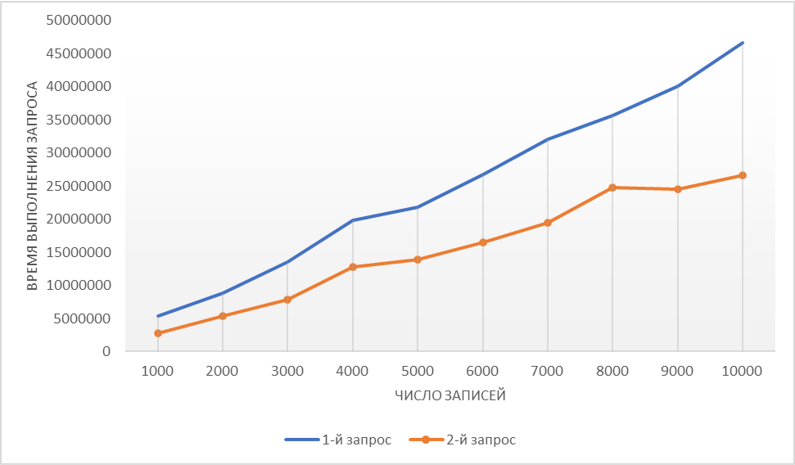
\includegraphics[scale=1.1]{inc/img/graph.png}
	\end{center}
	\captionsetup{justification=centering}
	\caption{\label{img:graph} Зависимость времени выполнения запросов от числа записей}
\end{figure}

%\clearpage

\subsection*{Выводы}
В данном разделе был проведён анализ времени выполнения двух видов запросов в зависимости от числа записей. 

В результате было выяснено, что время выполнения прямо пропорционально числу записей. Также было выяснено, что второй вариант запроса выполняется быстрее первого. За счёт усовершенствования запроса удалось снизить время выполнения в среднем примерно на 40,3\%.

Таким образом, на основании полученных данных можно сделать вывод, что на время выполнения запроса влияет как число записей в таблице, так и вид самого запроса.


\specsection{Заключение}

Цель курсового проекта достигнута. Спроектировано и реализовано программное обеспечение для поиска и бронирования репетиционных баз.

В ходе работы было формализовано задание, определён необходимый функционал, проведён анализ различных СУБД, спроектированы и реализованы база данных и приложение в соответствии с поставленной задачей, а также проанализировано время выполнения различных запросов к БД в зависимости от числа записей в таблицах.

Также в ходе выполнения поставленной задачи были изучены возможности языка Python и его расширения PyQt, получен опыт работы с PostgreSQL и pgAdmin, получены знания в области баз данных.

% говно литература для тест ВКР
\specsection{СПИСОК ИСПОЛЬЗОВАННЫХ ИСТОЧНИКОВ}

\begingroup
\renewcommand{\section}[2]{}
\begin{thebibliography}{}
	
\bibitem{subd_opr}
ISO/IEC TR 10032:2003 Information technology – Reference model of data management.

\bibitem{data_model}
Дейт К. Дж. Введение в системы баз данных. – 8-е изд. – М.: «Вильямс», 2006.

\bibitem{file_server}
Еленев Д. В. и др. Автоматизация системы управления национальным исследовательским университетом и мониторинга его деятельности // Программные продукты и системы, №3, 2012.

\bibitem{acid}
MySQL и модель ACID [Электронный ресурс]. -- Режим доступа: \url {https://spec-zone.ru/RU/mysql/5.6/storage-engines\_mysql-acid.html} (дата обращения: 02.06.2022).

\bibitem{python}
Yogesh Rana. Python: Simple though an Important Programming language // International Research Journal of Engineering and Technology (IRJET), 2019.

\bibitem{pyqt}
What is PyQt? [Электронный ресурс]. -- Режим доступа: \url {https://riverbankcomputing.com/software/pyqt/intro} (дата обращения: 04.06.2022).

\end{thebibliography}
\endgroup

% норм по феншую
%\bibliographystyle{utf8gost705u}
%\renewcommand{\refname}{СПИСОК ИСПОЛЬЗОВАННЫХ ИСТОЧНИКОВ}
%\bibliography{bibliography}

\anonsection{ПРИЛОЖЕНИЕ А}\label{app:signin}

\begin{lstlisting}[caption={реализация GUI окна входа/регистрации}]
	class Ui_MainWindow(object):
		def setupUi(self, MainWindow):
			MainWindow.setObjectName("MainWindow")
			MainWindow.resize(800, 600)
			self.centralwidget = QtWidgets.QWidget(MainWindow)
			self.centralwidget.setObjectName("centralwidget")
			self.signin_button = QtWidgets.QPushButton(self.centralwidget)
			self.signin_button.setGeometry(QtCore.QRect(240, 290, 161, 31))
			font = QtGui.QFont()
			font.setPointSize(12)
			self.signin_button.setFont(font)
			self.signin_button.setObjectName("signin_button")
			self.signup_button = QtWidgets.QPushButton(self.centralwidget)
			self.signup_button.setGeometry(QtCore.QRect(420, 290, 161, 31))
			font = QtGui.QFont()
			font.setPointSize(12)
			self.signup_button.setFont(font)
			self.signup_button.setObjectName("signup_button")
			self.label = QtWidgets.QLabel(self.centralwidget)
			self.label.setGeometry(QtCore.QRect(300, 250, 251, 20))
			font = QtGui.QFont()
			font.setPointSize(12)
			self.label.setFont(font)
			self.label.setObjectName("label")
			MainWindow.setCentralWidget(self.centralwidget)
			self.menubar = QtWidgets.QMenuBar(MainWindow)
			self.menubar.setGeometry(QtCore.QRect(0, 0, 800, 18))
			self.menubar.setObjectName("menubar")
			MainWindow.setMenuBar(self.menubar)
			self.statusbar = QtWidgets.QStatusBar(MainWindow)
			self.statusbar.setObjectName("statusbar")
			MainWindow.setStatusBar(self.statusbar)
			
			self.retranslateUi(MainWindow)
			QtCore.QMetaObject.connectSlotsByName(MainWindow)
\end{lstlisting}

\clearpage

\specsection{ПРИЛОЖЕНИЕ Б} \label{app:controller}

\begin{lstlisting}[caption={контроллер окна входа/регистрации}]
	class Welcome(QtWidgets.QMainWindow, welcome.Ui_MainWindow):
		def __init__(self):
			super().__init__()
			self.setupUi(self)
			self.signin_button.clicked.connect(self.sign_in)
			self.signup_button.clicked.connect(self.sign_up)
	
		def sign_in(self):
			self.window = SignIn()
			self.window.show()
	
		def sign_up(self):
			self.window = SignUp()
			self.window.show()
\end{lstlisting}

\clearpage

\specsection{ПРИЛОЖЕНИЕ В} \label{app:db}

\begin{lstlisting}[caption={подключение к БД с разными ролями}]
    def connect():
    	connection = None
    	try:
    		connection = psycopg2.connect(host="localhost", database="DB_course",
    		user="postgres", password="****")
    	except OperationalError as e:
    		print("The error '{e}' occurred")
    	return connection
    def connect_musician():
    	connection = None
    	try:
    		connection = psycopg2.connect(host="localhost", database="DB_course",
    		user="musician", password="****")
    		print("Connection of musician successful")
    	except OperationalError as e:
   			print("The error '{e}' occurred")
    	return connection
    def connect_owner():
    	connection = None
    	try:
    		connection = psycopg2.connect(host="localhost", database="DB_course",
    		user="base_owner", password="****")
    		print("Connection of owner successful")
    	except OperationalError as e:
    		print(f"The error '{e}' occurred")
    	return connection
    def connect_admin():
    	connection = None
    	try:
    		connection = psycopg2.connect(host="localhost", database="DB_course",
    		user="app_admin", password="****")
    		print("Connection of admin successful")
    	except OperationalError as e:
    		print(f"The error '{e}' occurred")
    	return connection
\end{lstlisting}

\clearpage

\specsection{ПРИЛОЖЕНИЕ Г} \label{app:proc}

\begin{lstlisting}[caption={процедура удаления реп. базы}]
    CREATE OR REPLACE PROCEDURE del_all(base_id int)
    AS $$
    	BEGIN
    	delete from rehearsal where roomid in (select id from room where baseid = base_id);
    	delete from equipment where roomid in (select id from room where baseid = base_id);
    	delete from room where baseid = base_id;
    	delete from reh_base where id = base_id;
    	END;
    $$ LANGUAGE PLPGSQL;
\end{lstlisting}

\clearpage

\specsection{ПРИЛОЖЕНИЕ Д} \label{app:dell_all}

\begin{lstlisting}[caption={применение процедуры при удалении реп. базы}]
	def del_base(conn, base_id):
		cur = conn.cursor()
		query = "CALL del_all(%s)"
		cur.execute(query, (base_id,))
		conn.commit()
		cur.close()
\end{lstlisting}


\end{document}
